\documentclass[11pt,twoside]{hsrthesis}

\makeindex


%add new glossaryentries here...

\newglossaryentry{sqlite}{
	name=SQLite,
	description={SQLite ist eine Datenbankengine, welche ohne Konfiguration auskommt. Es handelt sich dabei um eine Datenbank in einer Datei},
	first={SQLite}
}
\makeglossaries
\raggedbottom %http://blog.emeidi.com/2009/03/07/damit-latex-paragraphen-nicht-vertikal-auf-die-seite-verteilt/
\begin{document}

\newcommand{\thesistitle}{OSM Crosswalk Detection}
\newcommand{\thesisauthora}{Bühler Severin}
\newcommand{\thesisauthorb}{Kurath Samuel}
\newcommand{\thesisauthorc}{}
\newcommand{\professor}{Prof. Keller Stefan}
\newcommand{\thesistype}{Semesterarbeit}
\newcommand{\departement}{Abteilung Informatik}
\newcommand{\school}{Hochschule für Technik Rapperswil}
\newcommand{\term}{Herbstsemester 2015}
\newcommand{\thedate}{18. Dezember 2015}
\newcommand{\timeperiode}{16.09.2015 - 18.12.2015}
\newcommand{\workload}{240 Stunden, 8 ECTS pro Student}
\newcommand{\linktothesis}{https://github.com/geometalab/OSM-Crosswalk-Detection}

\setlength{\oddsidemargin}{20mm}
\maketitle
\setlength{\oddsidemargin}{20mm}

\section{Abstract}

Fussgängerstreifen sind ein essentieller Bestandteil der Fussgängernavigation. Sie sind jedoch nur spärlich in OpenStreetMap erfasst, was somit zu nicht optimalen Routen führt.

Um dem entgegen zu wirken,  befasst sich dieses Projekt mit der automatischen Erkennung von Fussgängerstreifen auf Orthofotos (Satellitenbildern). 
Dabei entstand eine hoch skalierbare Applikation, die gelbe Fussgängerstreifen entlang von Strassen findet und ihre Koordinaten extrahiert. Die Erkennung erfolgt durch ein Convolutional Neural Network, welches im Bereich des Deep Learnings angesiedelt ist.
Es wurde eine Erkennungsrate von über 80\% der visuell sichtbaren Fussgängerstreifen mit einer Fehlerrate von weniger als 10\% erreicht. Dieser Prozess konnte mit Hilfe eines Queueing Systems auf eine grosse Anzahl von Computern verteilt werden, was die Verarbeitung so vieler Daten in angemessener Zeit überhaupt erst ermöglichte. Die Koordinaten der Fussgängerstreifen wurden im Anschluss an das Crowdsourcing-System MapRoulette übergeben. Auf diesem Weg konnten die Daten in OpenStreetMap integriert werden und zur Verbesserung der Fussgängernavigation ihren Anteil beitragen.

Es ist möglich diese Lösung so auszubauen, dass der Erkennungsalgorithums auf weitere Objekte angewendet werden kann.

\section{Management Summary}
\subsection*{Ausgangslage}
Open Street Map, eine online Kartenanwendung wie Google Maps, bietet seinen Benutzern eine Fussgängernavigation an. Der Nutzer wird entlang von Strassen und Wegen zu seinem Ziel geleitet. Dabei müssen die bestehenden Fussgängerstreifen in die Planung einbezogen werden, damit auch eine Überquerung der Strassen möglich ist. Unglücklicherweise sind Zebrastreifen nur lückenhaft in Open Street Map erfasst, was die Fussgängernavigation ungenau, wenn nicht sogar fehlerhaft macht.

Dieses Projekt ist der Versuch einer automatischen Erkennung von Fussgängerstreifen auf Orthofotos (umgangssprachlich Satellitenbildern). Da das maschinelle Erfassen von Daten in Open Street Map nicht erlaubt ist, müssen die gefundenen Koordinaten in ein Crowdsourcing-System wie Maproulette eingespeist werden. In einem Crowdsourcing-System bewerten Nutzer, ob die eingefügten Daten stimmen oder nicht.
\begin{figure}[H]
	\centering
	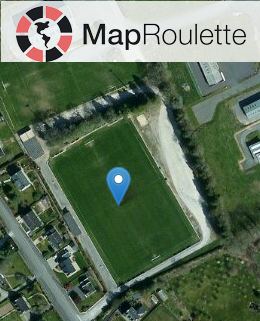
\includegraphics[]{images/Maproulette_management_summary.png}
	\caption[Management Summery Maproulette]{Maproulette Challenge - Befindet sich hier ein Fussballfeld?}
\end{figure}


\subsection*{Ergebnisse}
Aus diesem Projekt entstand einen Applikation für die automatische Erkennung von Fussgängerstreifen. Die Applikation bezieht in einem angegebenen Bereich automatisch die entsprechend Orthofotos und Strasseninformationen und extrahiert die Koordinaten der Fussgängerstreifen. Die Koordinaten werden in einer Json-Datei abgelegt und können in eine Maproulette Challenge umgewandelt werden.
\\
\begin{figure}[H]
	\centering
	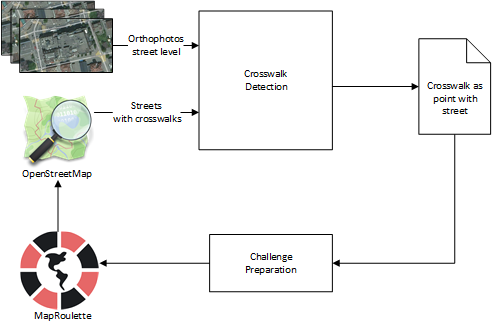
\includegraphics[]{images/management_summary_1.png}
	\caption[Management Summery Überblick]{Überblick}
\end{figure}

\subsubsection{Kennzahlen}
Die Applikation erkannte mehr als 80\% aller gelben Fussgängerstreifen mit einer Fehlerrate von weniger als 10\%. Die Koordinaten der Fussgängerstreifen im Raum des Kanton Zürich, Kanton Zugs und Teile des Kanton St. Gallen konnten an Maproulette zur Einpflegung in Open Street Map übergeben werden
\\
\begin{figure}[H]
	\centering
	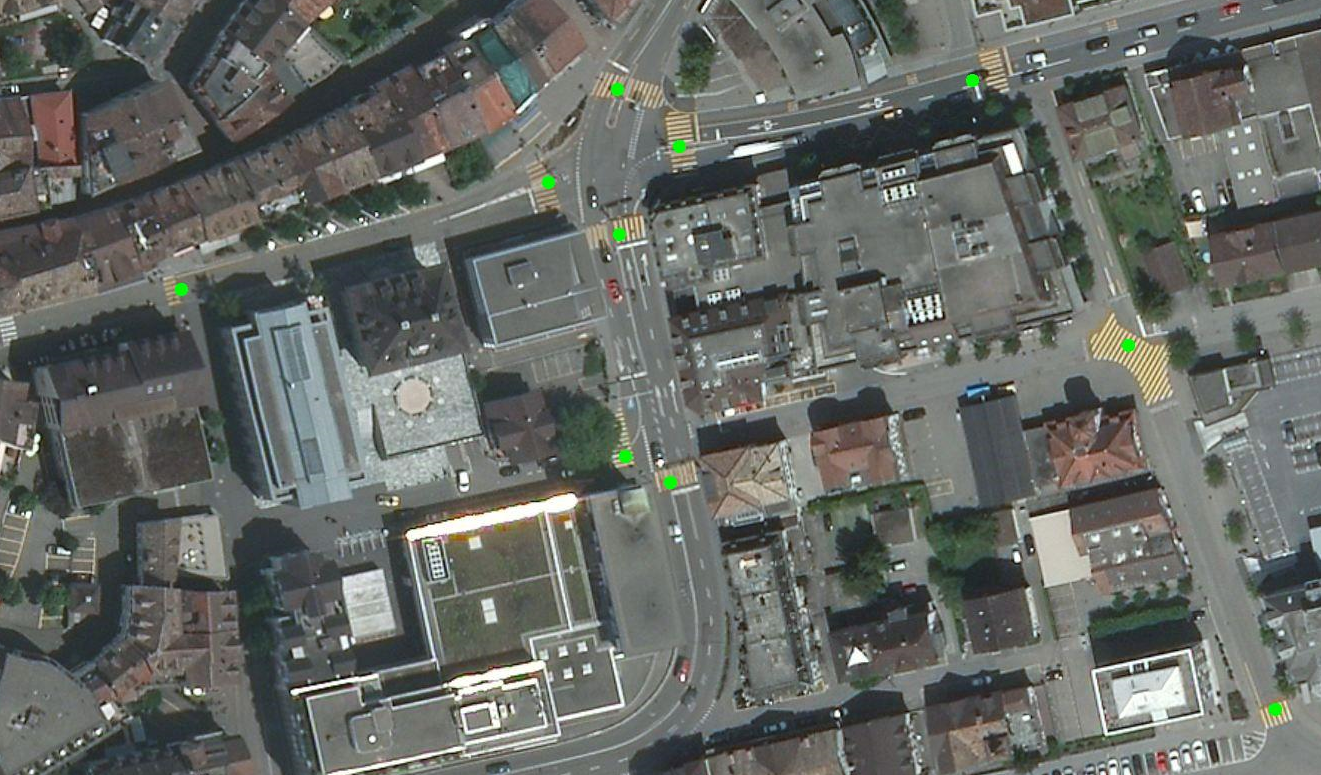
\includegraphics[width=\textwidth -10mm]{images/boxsave_rappi.png}
	\caption[Überblick]{Rapperswil Innenstadt - Gefundene Fussgängerstreifen sind mit einem grünen Punkt markiert.}
\end{figure}

\subsection*{Ausblick}
Der Erkennungsalgorithmus ist zu Ende dieses Projektes auf die Region Zürich und Ostschweiz spezialisiert. Mit weiteren Optimierungen ist es möglich, alle Zebrastreifen in der Schweiz zu erfassen und sogar weisse Zebrastreifen für andere europäische Länder zu erkennen. Auch weitere Strassenmarkierungen sind denkbar.
\newpage
\tableofcontents
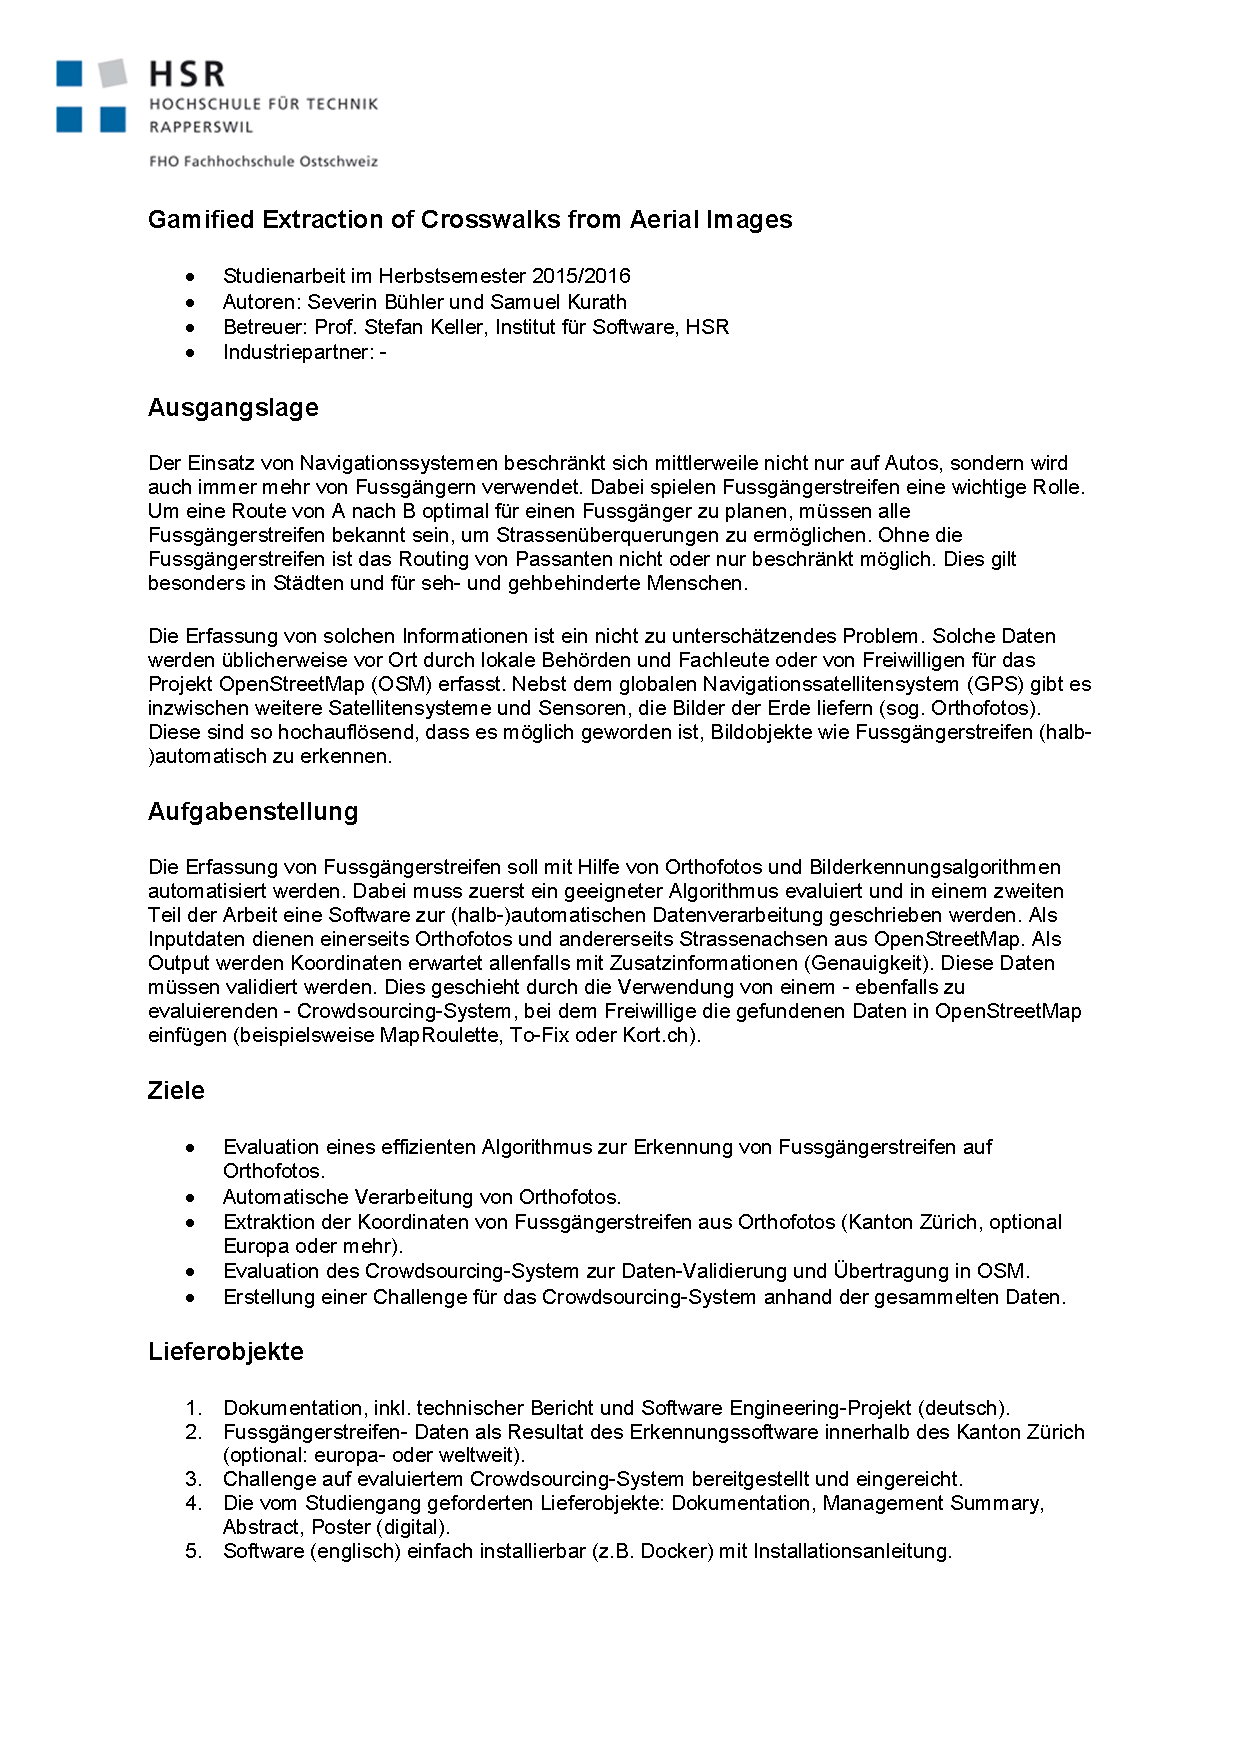
\includepdf[pages=-,frame,scale=.7,pagecommand={\section*{Aufgabenstellung}}]{pdfs/aufgabenstellung1.pdf}
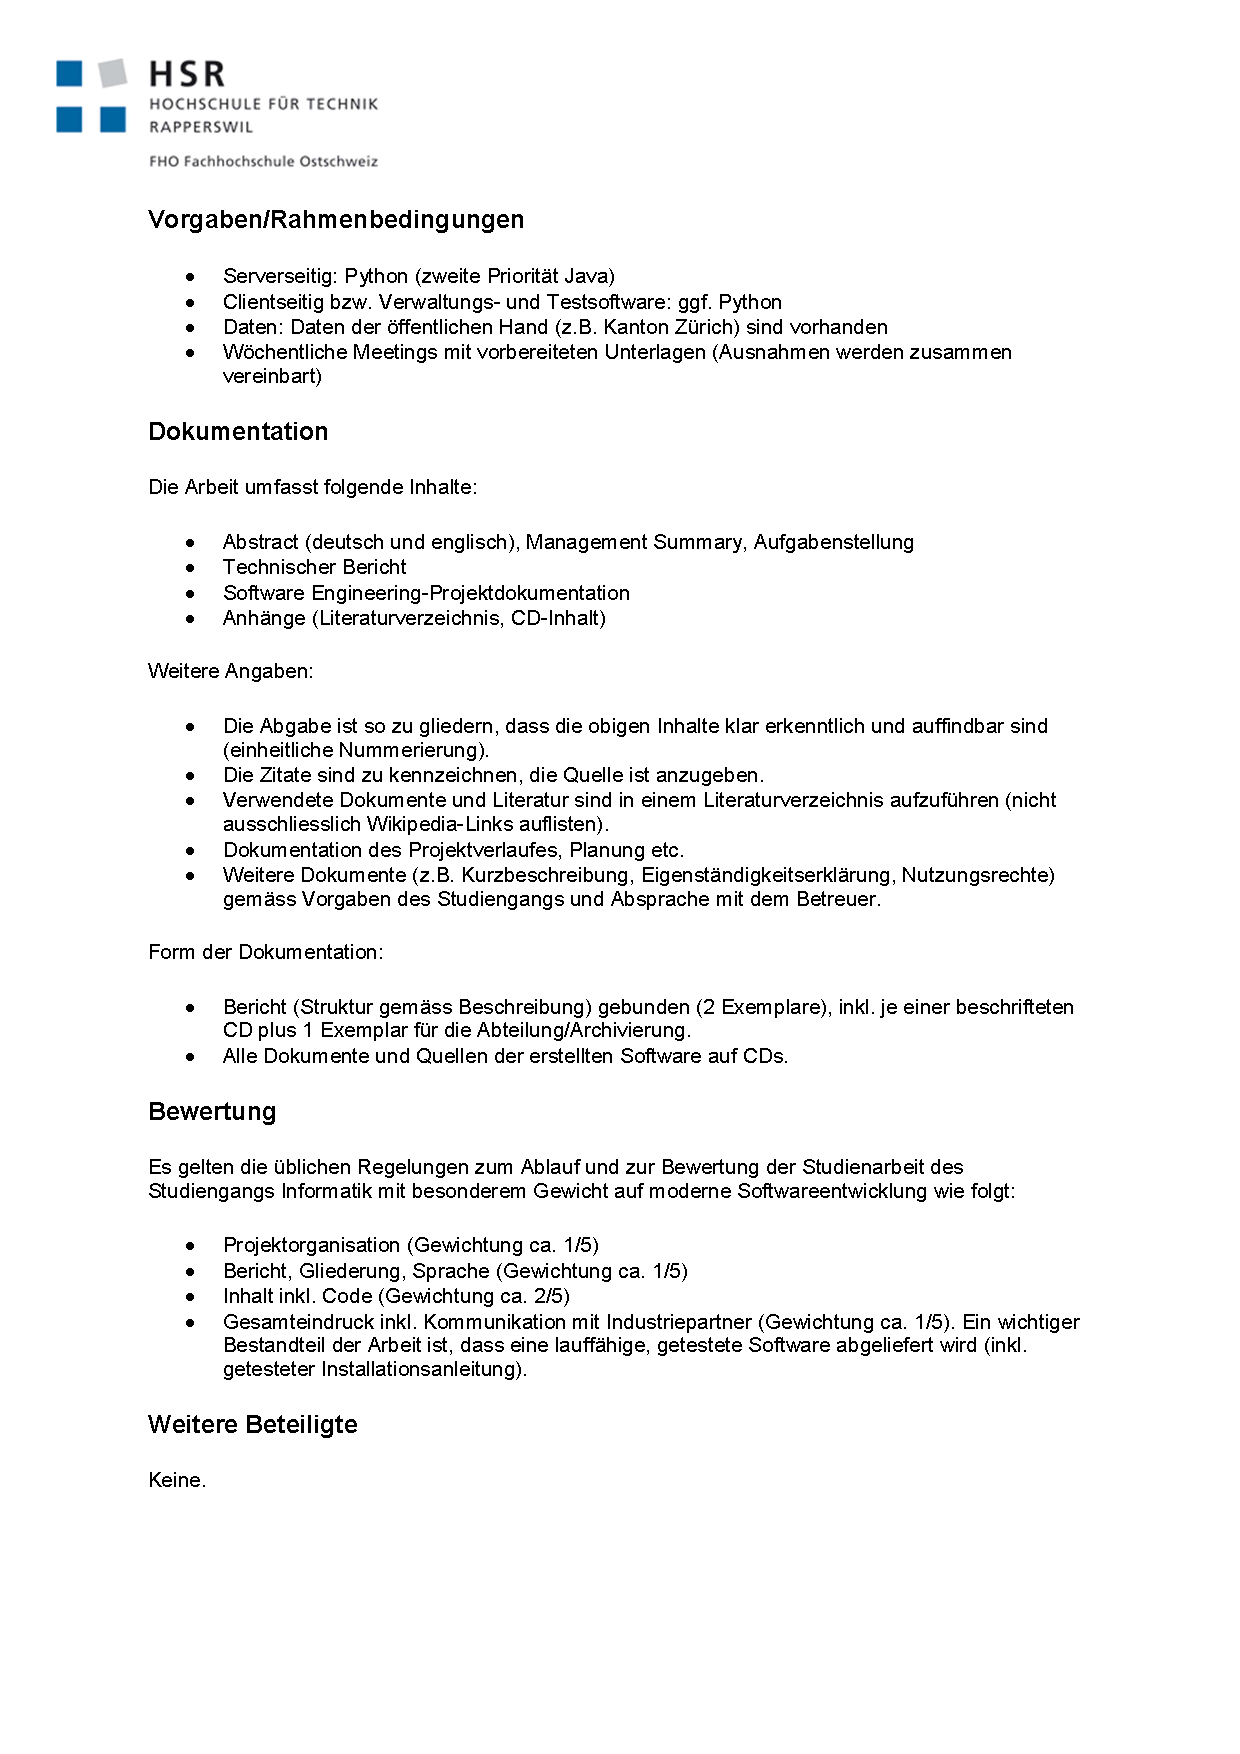
\includepdf[pages=-,frame,scale=.7,pagecommand={}]{pdfs/aufgabenstellung2.pdf}

% The main content
%%%%%%%%%%%%%%%%%%
\chapter{Technischer Bericht}
\section{Stand der Technik}
Um abzuklären, ob es schon Arbeiten gab, die ähnliche Probleme lösen, nahmen wir uns im Rahmen der Semesterarbeit Zeit für ein Literaturrecherche. Dabei gingen wir auf die HSR Bibliothek und deren Mitarbeiter zu.
\subsection{Literaturrecherche}
\subsubsection{Suchquellen}
Folgende Quellen wurden uns empfohlen, um Recherchen in diesem Umfeld durchzuführen:
\begin{itemize}
	\item NEBIS \cite{NEBIS}
    \item IEEXplore \cite{IEEXplore}
    \item Google Scholar \cite{GoogleScholar}
\end{itemize}

\subsubsection{Auswertung}
Bei der Recherche stiessen wir auf verschiedene Projekte, die sich mit der Problematik des Erkennens von Fussgängerstreifen auseinander setzen. Leider sind diese Arbeiten eher im Bereich der Bilderkennung für die Steuerung von autonom fahrenden Autos/Robotern angesiedelt. Arbeiten die treffender sind, werden im Anschluss angeführt.
\subsubsection{Extraction of Road Markings from Aerial Images}
Yuichi Ishino und Hitoshi Saji (Japan, 2008)\cite{ishino2008extraction} \newline 

An der Univerisität Shizuoka in Japan gab es vor einigen Jahren eine Arbeit zur Erkennung von Fussgängerstreifen und Mittellinien (Traffic Lane Lines) auf Orthofotos (Aerial images).

Ihr Algorithmus befolgt dabei folgende Strategie:
Der Algorithmus geht den Strassen entlang und richtet die Bilder so aus, dass die Fussgängerstreifen immer vertikal zur Achse laufen. Danach wird eine sogenannte Binarization durchgeführt. Es setzt alle Pixel unter einem Schwellwert auf 0 (weiss) und alle Pixel darüber auf 1 (schwarz). Es wurden zwei Schwellwerte zuvor berechnet, einmal für sonnige und einmal für schattige Bilder.
Mit den Annahmen, dass die Strasse schwarz/grau und der Fussgängerstreifen leuchtend weiss sind, sieht man nun ein gleichmässiges Muster in der Helligkeitsverteilung des Bildes. Ein Fouriertransformation würde eine saubere Frequenz liefern.

Die Arbeit von Ishino und Saji geht von einigen Grundannahmen und Vorraussetzungen aus, die die Erkennung sehr erleichtern:

\begin{itemize}
	\item Die Fussgängerstreifen sind immer gerade und werden durch keine Inseln unterbrochen.
	\item Die Auflösung der Bilder ist genug gross, um das Streifenmuster ohne Probleme zu erkennen.
	\item Der Fussgängerstreifen ist immer deutlich heller als die Strasse selbst.
	\item Der Streifen werden durch keine Hindernisse wie Bäume, Autos verdeckt oder beeinflusst.
	\item Die Bilder wurde zuvor in die Kategorien schattig und sonnig eingeteilt worden. Auf ihnen wird mit verschiedenen Schwellwerten gearbeitet.
	\item Die Strassen müssen die Fussgängerstreifen immer vertikal schneiden.
\end{itemize}

\paragraph{Schlussfolgerung}
Die Arbeit der Universität von Shizuoka verfolgte einen ähnlichen Ansatz, den wir mit der Fouriertransformation in Betracht ziehen. Leider gehen die Dokumentverfasser von einigen Grundannahmen aus, die sich nicht mit der unseren Arbeit decken. Man kann fast schon von Laborbedingungen sprechen.
Doch gibt es einigen Techniken, die sich auch für unsere Arbeit verwenden lassen. Diese sind unten aufgeführt.

\subsubsection{Segmentation of Occluded Sidewalks in Satellite Images}
Turgay Senlet und Ahmed Elgammal, The State University of New Jersey, USA (2012)\cite{senlet2012segmentation} \newline

Das Projekt von Turgay Selent und Ahmed Elgammal setzte sich mit der Erkennung von primär Gehwege (sidewalks) und Fussgängerstreifen auf Satellitenbildern auseinander.

Dabei waren die Hauptprobleme, dass viele Gehwege von Bäumen oder Schatten verdeckt werden. Um diesem Problem Herr zu werden, benutzten sie einen Farbklassifizierer.
Um Fussgängerstreifen zu klassifizieren, stellten sie eine Sammlung an Frequenzen in allen möglichen Winkeln zusammen. 

Leider wird im Artikel zu dieser Arbeit nicht weiter auf die Erkennungsmethoden eingegangen.

\subsubsection{Fazit}
Aus allen Arbeiten konnten wir doch einige Techniken finden, die uns die Erkennung erleichtern könnten. Diese sind hier aufgelistet:
\begin{itemize}
	\item Binarization image 
	\item Median Filter (für Verbesserung der Bildqualität von ungenauen Bildern)
\end{itemize}

\newpage
\section{Evaluation Crowdsourcing-System}
\label{sec:crowdsourcing}
Da Daten nicht automatisch in OpenStreetMap integriert werden dürfen, wird ein Crowdsourcing-System benötigt. In diesem überprüfen Benutzer auf spielerische Art und Weise, ob die Daten korrekt sind.\\
Es gibt verschiedene Produkte in diesem Bereich, somit haben wir als Teil unserer Arbeit eine Evaluation zweier relevanter Kandidaten durchgeführt.
\subsubsection{Kandidaten}
\begin{itemize}
	\item MapRoulette \cite{MapRoulette}
	\item To-Fix \cite{To-Fix}
\end{itemize}

\subsection{MapRoulette}
\label{subsec:MapRoulette}
\Gls{MapRoulette} verwendet für ihre Challenges und Tasks ein einfaches JSON Format. Erstellt werden Challenges mittels POST und mit PUT können diese upgedatet werden.

\subsubsection{Beispiel Challenge}
\begin{tabbing}
    \hspace*{4cm}\=\hspace*{5cm}\= \kill
    Erstellen: \> POST /api/admin/challenge/<slug>  \\
    Updaten: \> PUT /api/admin/challenge/<slug> \\
    Challenge JSON: \\
\end{tabbing}		
\begin{python}
{
  "title": "Repair Motorways",
  "description": "Repair all motorways",
  "blurb": "The idea is to repair all motorways",
  "help": "Repair the ways where it is broken on the map",
  "instruction": "Look at the map for broken pieces.",
  "active": true,
  "difficulty": 2
}
\end{python}
\newpage
\subsubsection{Beispiel Task}
\begin{tabbing}
    \hspace*{4cm}\=\hspace*{5cm}\= \kill
    Erstellen: \> POST /api/admin/challenge/<slug>/task/<task\_identifier> \\
    Updaten: \> PUT /api/admin/challenge/<slug>/task/<task\_identifier> \\
    Challenge JSON: \\
\end{tabbing}
\begin{python}
{ 
  "instruction" : "This is a hard task!",
  "geometries" : {
    "type": "FeatureCollection",
    "features": [
      { "type": "Feature",
        "geometry": 
        { "type": "Point", 
          "coordinates":[-41.4710170873565,31.235521774136]
        },
        "properties": {"osmid": 12345}
      }
    ]
  }
}
\end{python}	

\subsection{To-Fix}
\Gls{To-Fix} verwendet für ihre Tasks ein CSV Format, welches direkt über das grafische Benutzerinterface publiziert werden kann.
\subsubsection{Beispiel CSV}
\begin{python}
object_type,object_id,st_astext
way,51446110,POINT(-94.4176451 43.3273692)
way,187403368,POINT(32.9369086 2.1997495)
way,220866128,POINT(-68.5 49.647521)
way,223982938,POINT(18.4823301 59.6732909)
way,109819283,POINT(-83.1888421 40.0485764)
\end{python}

\newpage

\subsection{Auswertung}
Um die beiden Kandidaten zu vergleichen, haben wir eine Evaluationsmatrix erstellt. Dabei haben wir diverse für uns relevante Kriterien erarbeitet und diese jeweils auf einer Skala von 1 bis 10 gewichtet.
In einem zweiten Schritt haben wir den Kandidaten für die jeweiligen Kriterien Punkte vergeben.\\

\begin{table}[H]
	\centering
    \begin{tabular}{|l|l|l|l|l|l|}
    \hline    
    \rowcolor{lightblue}
    Kriterium & Gewicht & Maproulette & Resultat &To-Fix & Resultat\\ \hline
	Challenge ist leicht erstellbar & 5 & 6 & 30 & 7 & 35 \\ \hline
	Challenge ist leicht publizierbar & 7 & 8 & 56 & 8 & 56 \\ \hline
	Anbieter ist relevant bei der Community & 8 & 8 & 64 & 4 & 32 \\ \hline
	Dokumentation & 7 & 5 & 35 & 5 & 35 \\ \hline
	Kontaktperson & 5 & 5 & 25 & 6 & 30 \\ \hline
	\rowcolor{lightblue} Total & 32 & 32 & 210 & 30 & 188 \\ \hline
    \end{tabular}    
    \caption[Evaluationsmatrix]{Evaluationsmatrix}
\end{table}

\decision{Crowdsourcing-System}
Beide Kandidaten haben Vor- und Nachteile, wie aus der Evaluationsmatrix ersichtlich ist. Für uns ist das wichtigste Kriterium, wie relevant der Anbieter bei der Community ist, was sich dann auch im Resultat stark ausgewirkt hat. Da MapRoulette Challenges gerne abgearbeitet werden, haben wir uns für diesen Kandidaten entschieden	
\chapter{Software Projektdokumentation}
\newpage 
\section{Einführung}
\subsection{Vision}
\label{subsec:vision}
\paragraph{Aktuell}
Die Navigation von Fussgänger wird immer beliebter, dabei spielen Fussgägnerstreifen ein wichtige Rolle. Leider sind diese nur spärlich erfasst. Auch die Behörden selbst haben keine kompletten Daten zu den Standorte. So hat zum Beispiel die Stadt Zürich das Projekt Zebra-Safari lanciert bei dem bis Ende 2016 alle Fussgängerstreifen erfassen und beurteilen werden sollen. Dieser Vorgang ist jedoch sehr arbeitsintensiv und wird händisch durchgeführt.\\

\paragraph{Vision} 
Es soll eine Applikation entstehen, mit der die aufwändige Problematik der Erfassung der Fussgängerstreifen automatisiert werden kann. Dies soll mit Hilfe von Bilderkennungsalgorithmen auf Orthofotos (Satellitenbildern) ermöglicht werden. 
\section{Anforderungsspezifikation}
\subsection{Use Case}
\subsubsection{Aktoren und Stakeholder}
\begin{table}[H]
\centering
    \begin{tabular}{|p{3cm}|p{9cm}|}
    \hline
    \rowcolor{lightblue}
    Aktor & Tätigkeit   \\ \hline
	User  & Startet CrosswalkDetector mit Bounding Box als Eingabeparameter \\ \hline
	CrosswalkDetector & Erkennt Fussgängerstreifen \\ \hline 
	TileProvider & Stellt Orthofotos für die Erkennung der Fussgängerstreifen zur Verfügung.\\ \hline
	OSMProvider & Stellt Strassen - und Fussgängersteifen Informationen zur Verfügung. \\ \hline
	JSON File & Speicherort für die Positionen der ermittelten Fussgängersteifen.\\ \hline
    \end{tabular}
    \caption[Aktoren und Stakeholder]{Aktoren und Stakeholder}
\end{table}

\subsubsection{Use Case Diagramm}
\begin{figure}[H]
\centering
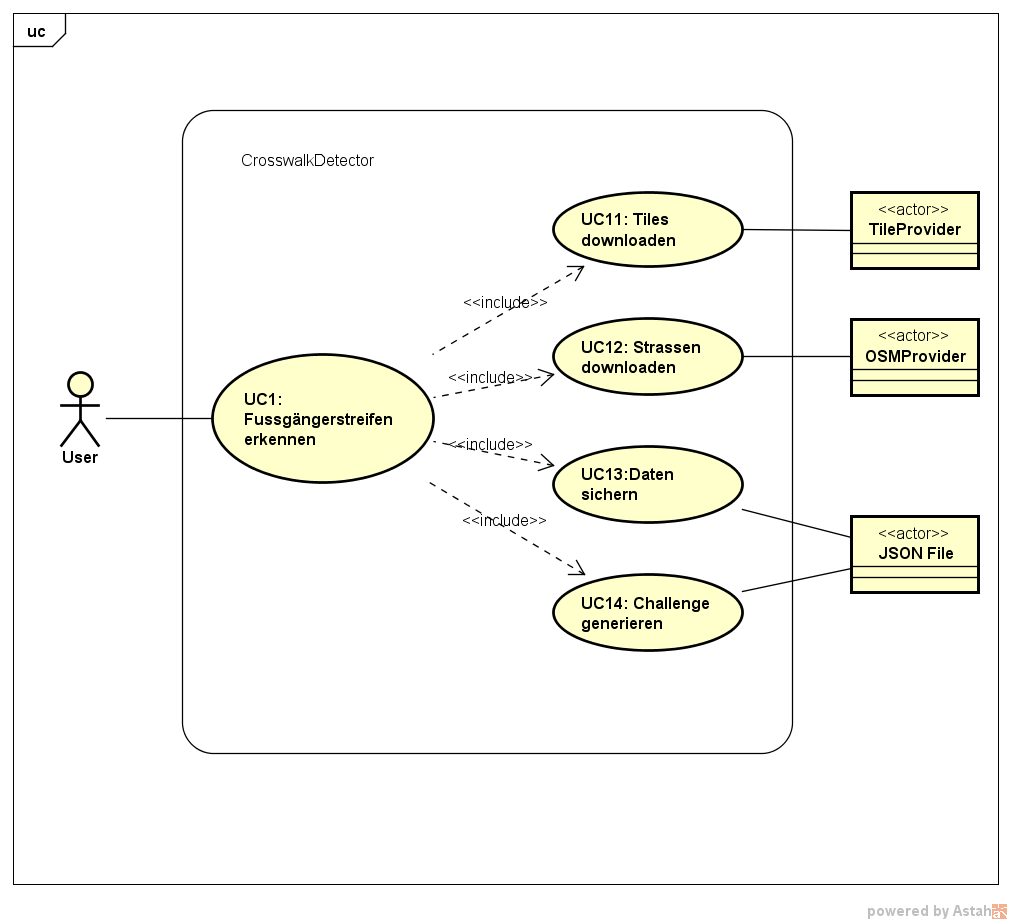
\includegraphics[width=420pt]{images/UseCase.png}
\caption[Use Case Diagramm]{Use Case Diagramm}
\end{figure}

\subsubsection{Use Cases Brief}
\paragraph{UC1: Fussgängerstreifen erkennen}
Der User startet die Applikation und gibt als Eingabeparameter ein Bounding Box an, welche nach Fussgängerstreifen durchsucht wird. Dabei werden Orthofotos mit Hilfe eines Erkennungsalgortithmus abgearbeitet.

\paragraph{UC11: Tiles downloaden} 
Ein TileProvider stellt Orthofotos zur Verfügung, welche heruntergeladen werden müssen. Diese werden im Anschluss dem Erkennungsalgorithmus zur Verfügung gestellt.

\paragraph{UC12: Stassen downloaden}
Ein OSMProvider stellt Informationen zu Strassen und Fussgängerstreifen zur Verfügung, welche vom Erkennungsalgorithmus genutzt werden. Mit diesen Daten kann die Suche präzisiert werden, sowie der Download von Orthofotos reduziert werden.

\paragraph{UC13: Daten sichern}
Die erkannten Fussgängerstreifen werden in einer JSON Datei persistiert. Dabei sind die Positionen (Koordinate lat/lon) relevant.

\paragraph{UC14: Challenge generieren}
Mit Hilfe der persistieren Daten wird ein Challenge generiert, welche die Daten über eine Crowdsourcing-System in OpenStreetMap integriert.

\subsubsection{Use Cases Fully Dressed}
\begin{table}[H]
    \begin{tabular}{ | p{4cm} | p{10cm}  | }
    \hline
    Scope & CrosswalkDetection System   \\ \hline
	Level  & User Goal \\ \hline
	Primary Actor & User \\ \hline 
	Stakeholders & 
	\begin{itemize}
		\item System: Möglichst alle Fussgängerstreifen erkennen
		\item User: Einmal gestartet, läuft alles autonom
    \end{itemize} \\ \hline
	Preconditions & 
		\begin{itemize}
		\item User muss Bounding Box bestimmen
		\item OSMProvider muss verfügbar sein
		\item TileProvider muss verfügbar sein
    \end{itemize} \\ \hline
	Postconditions & Koordinaten der Fussgängerstreifen persistiert \\ \hline
	Main Success Scenario & 
	\begin{enumerate}
		\item CrosswalkDetection wird mit Angabe der Boundingbox aufgerufen
		\item Daten von OSMProvider werden heruntergeladen
		\item Orthofotos von TileProvider werden heruntergeladen
		\item Erkennungsalgorithums erfasst Fussgängerstreifen
		\item Daten sind persistiert
	\end{enumerate} \\ \hline
	Extensions & 
	\begin{enumerate}
		\item a) Bounding Box wird aufgeteilt für Parallelisierung
		\item b) Nur Informationen für Strassen und Fussgängerstreifen sind relevant
		\item b) Nur Orthofotos, welche Strassen beinhalten, werden heruntergeladen.
	\end{enumerate} \\ \hline
	Special Requirements & Benutzer soll gut geführt werden und bei Unklarheiten
von Parametern Informationen erhalten. \\ \hline
	Frequency of Occurrence & Der Vorgang darf beliebig oft wiederholt werden. \\ \hline
	Open Issues & Falls ein Unterbruch statt findet, soll von diesem Zustand weiter gearbeitet werden. \\ \hline
    \end{tabular}
    \caption[Use Case Fully Dressed]{Use Case Fully Dressed}
\end{table}



\newpage
\subsection{Sequenzdiagramm}
\subsubsection{Queueing}
Das Queueing Sequenzdiagramm beschreibt den Parallelisierungprozess.
\begin{figure}[H]
	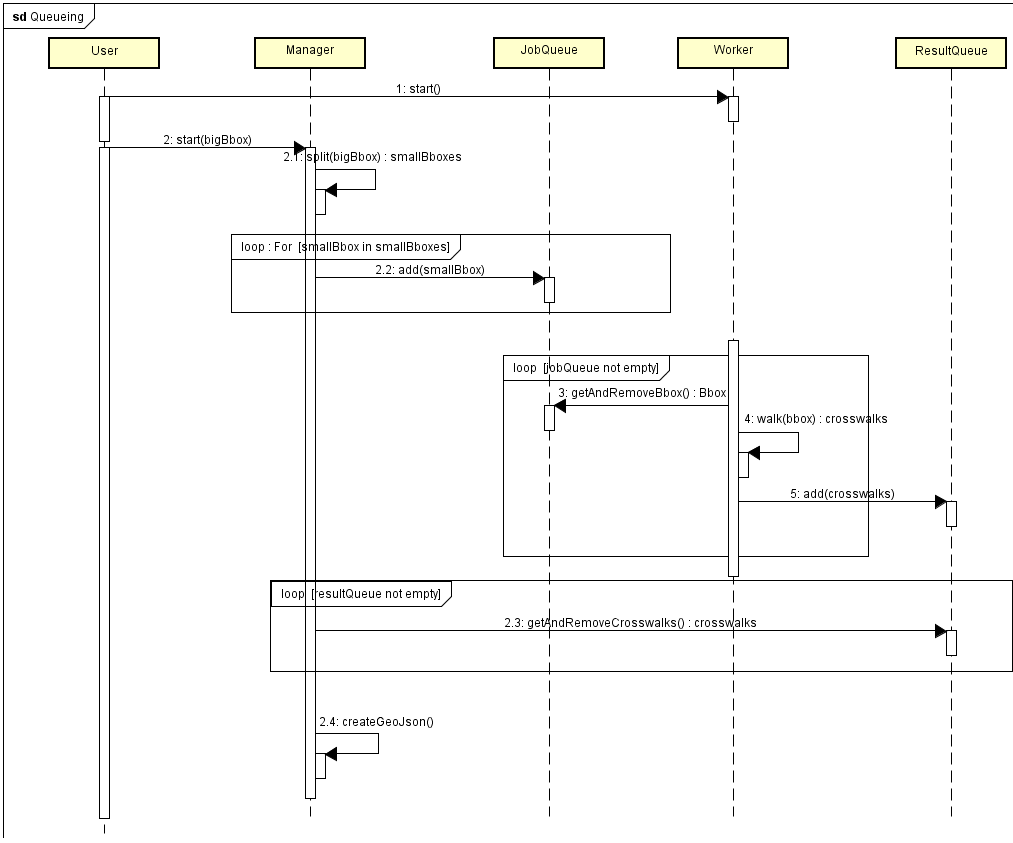
\includegraphics[width=\textwidth]{images/seq_queueing.png}
	\caption{Sequenzdiagramm Queueing}
\end{figure}

\newpage
\subsubsection{Walking}
Das Walking Sequenzdiagramm beschreibt den Ablauf, wie eine Bounding Box von einem JobWorker abgearbeitet wird.
\begin{figure}[H]
	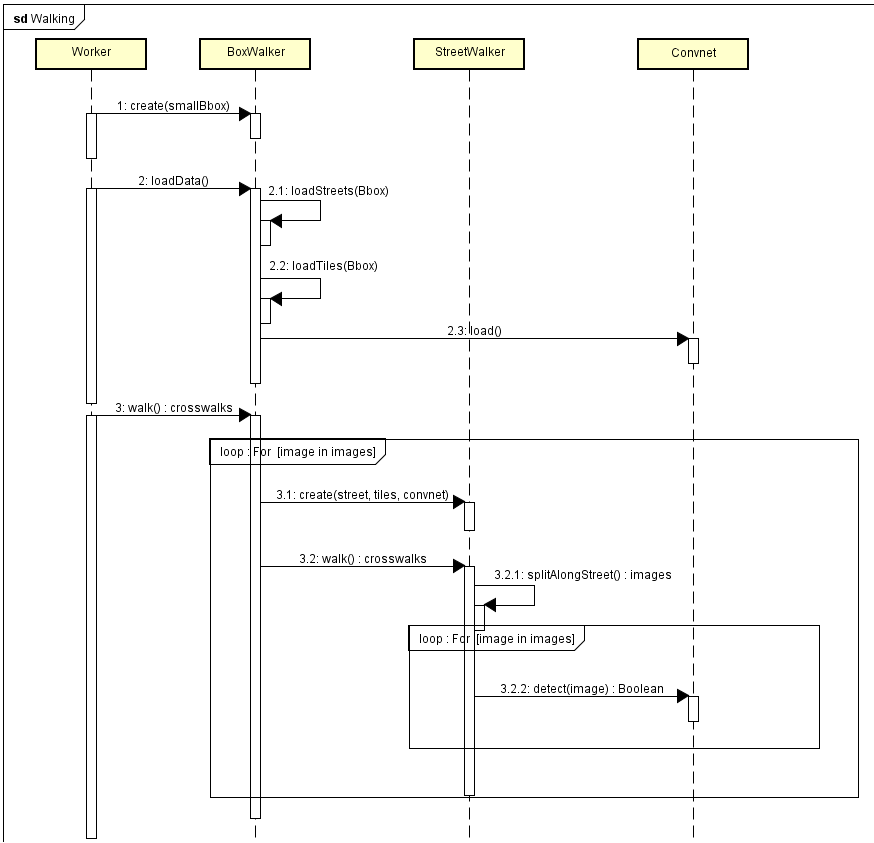
\includegraphics[width=\textwidth]{images/seq_walking.png}
	\caption{Sequenzdiagramm Walking}
\end{figure}
\subsection{Nichtfunktionale Anforderungen}
\subsubsection{Funktionalität}
\paragraph{Sicherheit}
Sicherheitsaspekte müssen nicht beachtet werden, es wird nicht mit Personen- oder stark Schützenswertendaten gearbeitet. Der Sourcecode steht unter der MIT Lizenz und ist auf Github verfügbar. Weiter werden die gesammelten Daten über OpenStreetMap für jederman zugänglich.
\paragraph{Interoperabilität}
Das System ist auf Orthofotos, sowie Strassen- und Füssgängerinformationen angewiesen.
Dazu stehen folgende API zur auswahl:
\begin{itemize}
	\item Bing Static Map Data
	\item Google Static Map API
	\item MapQuest API
	\item Overpass
\end{itemize}

\paragraph{Richtigkeit}
Die Richtigkeit der erkannten Fussgängerstreifen wird mit Hilfe eines Crowdsourcing-Systems sichergestellt. Dabei verifizieren Freiwillige die erkannten Fussgängerstreifen.
\subsubsection{Zuverlässigkeit}
\paragraph{Wiederherstellbarkeit}
Nach einem Systemabsturz oder Stopp der Anwendung, soll die Anwendung ohne Komplikationen wieder gestartet werden können. Beim Neustart soll ab der Absturzstelle weitergearbeitet werden können, ohne das Daten oder bis anhin erbrachte Rechenleistungen verlohren gehen.
\paragraph{Fehlertoleranz}
Fehler in einzelnen Jobs sollen keine Systemweiten auswirkungen haben. Jede Operation soll im Fehlerfall wiederholt werden können.
\paragraph{Availability}
Bei Nichtverfügbarkeit des Systems entsteht kein direkter finanzieller Schaden, deshalb ist die Systemverfügbarkeit nicht von oberster Priorität. 
\subsubsection{Benutzbarkeit}
Die Benutzung der Anwenung beschränkt sich auf die Eingabe der Bounding Box für den Bereich an dem Fussgängerstreifen erkannt werden sollen. Ansonsten soll keine Interreakton mit dem Benutzer statt finden. Auf eine grafische Oberfläche wird verzeichte, es ist ein reine Konsolenapplikation.

\paragraph{Robustheit}
Die Eingabe der Bounding Box durch den Benutzer muss auf Korrektheit überprüft werden. Da die Applikation sehr rechenintensiv ist, soll bei einem Absturz, an der Absturz stelle weiter gearbeiten werden können.
\subsubsection{Effizienz}
Eine Erkennungsrate von 80% wird angestrebt.
Schnittstellen:
\begin{itemize}
	\item Bing Static Map Data
	\item Google Static Map API
	\item MapQuest API
	\item Overpass
\end{itemize}

\subsubsection{Supportability}
\paragraph{Internationalization}
Das System sollte vorerst nicht verschiedene Sprachen unterstützen. 
Die Standardsprache ist Englisch.



\subsection{Analyse}
\begin{figure}[H]
	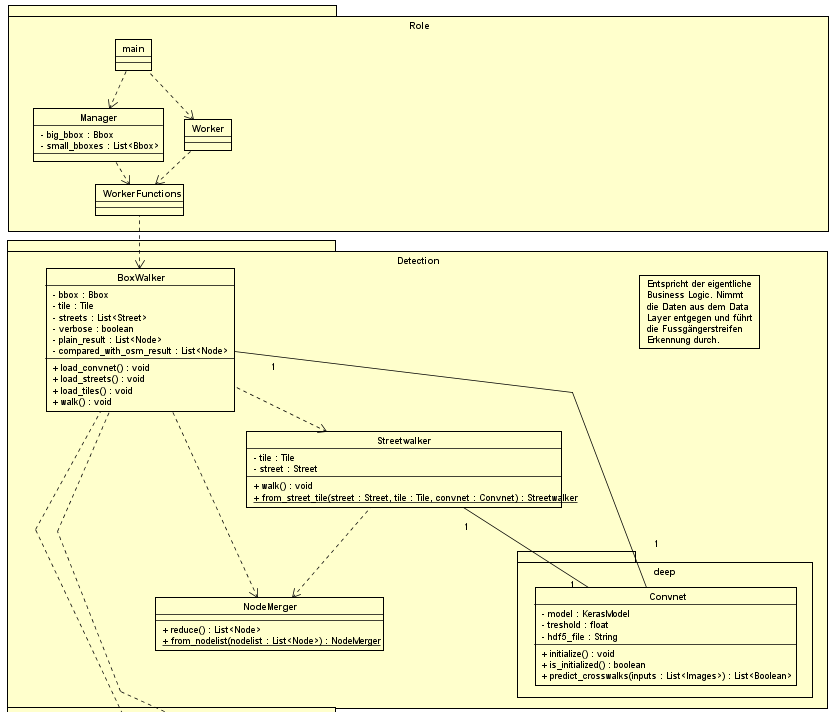
\includegraphics[width=\textwidth]{images/domain_model_komplett1.png}
	\caption{Domain Modell Teil 1}
\end{figure}
\begin{figure}[H]
	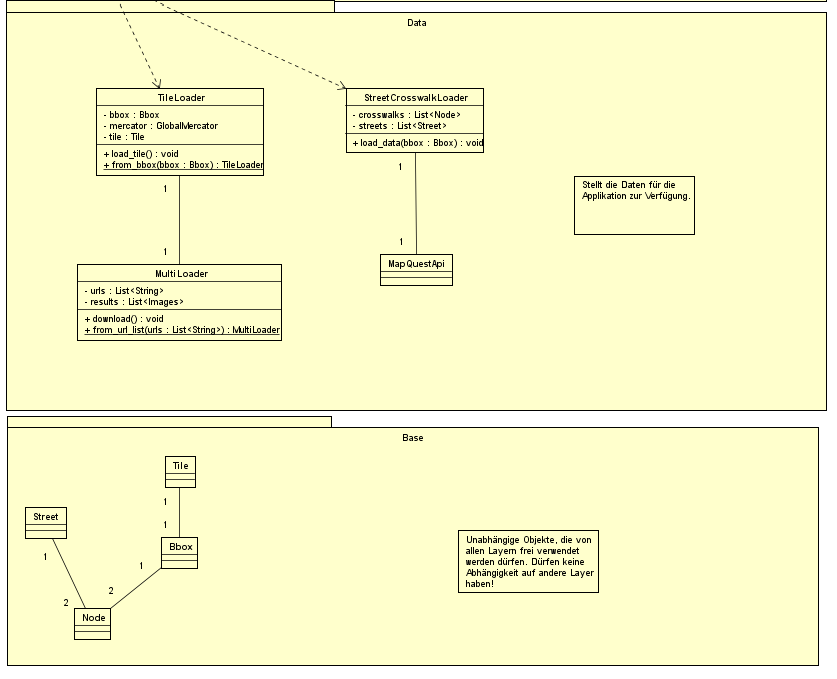
\includegraphics[width=\textwidth]{images/domain_model_komplett2.png}
	\caption{Domain Modell Teil 2}
\end{figure}
\subsubsection{Beschreibung Domain Modell}
Das Domain Modell besteht aus 4 Layern welche von oben nach unten auf einander aufbauen. Die Packages im Projekt sind gleich benannt wie die Layer. Die genauen Funktionen der entsprechenden Klassen sind im Kapitel Implementation einzusehen.
\begin{enumerate}
	\item Role - Parallelisierung
	\item Detection - Bilderkennung
	\item Data - Dataprovider
	\item Base - Grundelemente
\end{enumerate}

\subsubsection{Base}
Der Base Layer stellt Grundklassen wie ein Node oder eine Street zur Verfügung. Dieser Layer weisst nur Abhängigkeiten zu verwendeten Bibliotheken auf.

\subsubsection{Data}
Der Data Layer stellt den klassichen Data Link Layer dar. Er stellt Klassen zur Verfügung, um auf die entsprechenden Daten zuzugreifen. In unserem Fall sind es Orthofotos und OpenStreetMap Daten. Dieses Package benutzt den Base Layer.

\subsubsection{Detection}
Der Detection Layer beinhaltet die Funktionen zur eigentliche Bilderkennung. Dieser Layer holt seine Daten aus dem Data Layer und benutzt den Base Layer.

\subsubsection{Role}
Der Role Layer managt die Parallelisierung. Er greift ausschliesslich auf den Detection und auf den Base Layer zu.
\\
\decision{Main Datei}
Die Main Datei ist hier speziell zu erwähnen. Main verwaltet die Kommandozeilenaufrufe und startet das Programm dementsprechend. Diese Datei sollte eigentlich in einem eigenen Presentation Layer sein. Da wir jedoch keinen separaten Layer nur für eine Klasse machen, haben wir Main in den Role Layer verschoben.

\section{Implementation}
Der Implementationsteil ist wie das Projekt selbst in 3 Teile aufgesplittet.
\begin{enumerate}
	\item Data Access - data
	\item Bilderkennung - detection
	\item Parallelisierung - role
\end{enumerate}
\subsection{Data Layer}
Der Data Accss Layer regelt den Zugriff auf die Orthofotos mit Bing Maps, sowie die Strassen und Fussgängerstreifen, welche mit Hilfe von OpenStreetMap Daten über die MapQuest API zur Verfügung gestellt werden. Die Daten werden von den entsprechenden Quellen heruntergeladen und für die Detektion zu einem passenden Format aufbereitet.

\subsubsection{MapQuest}
\Gls{MapQuest}\footnote{\url{http://www.mapquest.com/}} wird in diesem Projekt als Schnittstelle zu den OpenStreetMap Daten verwendet. Dazu bieten sich die Developer Accounts an, welche auf 15000 Abfragen pro Monat begrenzt sind, was unseren Abfrageumfang ausreichend abdeckt.
Folgende Daten benötigen wir von der API:
\begin{tabbing}[H]
    \hspace*{3cm}\=\hspace*{9cm}\= \kill
    Strassen: \> Der Suchalgorithmus folgen den Strassenverläufen, \\
     			\> was die Suche effizienter und einfach werden lässt.\\
    Fussgängerstreifen: \> Schon erfasste Fussgängerstreifen werden mit den von uns  \\ \> Entdeckten verglichen und nur diejenigen, welche noch nicht in erfasst sind,\\ \> werden abgespeichert.
\end{tabbing}


\subsubsection{Application Key}
In der Tabelle ist der Application Key aufgeführt, der für das Projekt Crosswalk Deteciton eingesetzt wurde.
\begin{table}[H]
	\begin{tabular}{ | p{6cm} | p{6cm}  | }
		\hline    
		Consumer Key &  YKqJ7JffQIBKyTgALLNXLVrDSaiQGtiI \\ \hline
		Consumer Secret & 3DO1eoLMxSqPH7Gk \\ \hline
		Key Issued & Fri, 09/25/2015 - 07:17 \\ \hline
		Key Expires & Never \\ \hline
	\end{tabular}
	\caption[MapQuest Application Key]{MapQuest Application Key}
\end{table}

\paragraph{Beispiel Abfragen}
Um den Entwicklern beim erstellen der Abfragen zu unterstützen wird folgende Webseite zur Verfügung gestellt:
\begin{itemize}
	\item \url{http://open.mapquestapi.com/xapi/}
\end{itemize}

\subparagraph{HTTP Request}
Bounding Box:  47.367,8.545,47.367,8.544 (Rapperswil)
\begin{itemize}
	\item \url{http://open.mapquestapi.com/xapi/api/0.6/node[highway=*][bbox=8.544,47.367,8.545,47.367]?key=YKqJ7JffQIBKyTgALLNXLVrDSaiQGtiI}
\end{itemize}


\subparagraph{XML File Response}
Als Antwort auf den HTTP Request gibt es ein XML File, welches die Strassen in Form von Nodes beinhaltet.\\

\begin{python}
	<osm xmlns:xapi="http://jxapi.openstreetmap.org/">
	<node id="32860913" version="8"
	timestamp="2015-08-06T15:21:13Z" uid="6087"
	lat="47.2254172" lon="8.8175171">
	<tag k="highway" v="traffic_signals"/>
	</node>
	</osm>
\end{python}



\paragraph{Abfrage}
Um das Resultat einer Abfrage einzugrenzen, bietet die API diverse Parameter und Tags die angegeben werden können. Damit wir nicht zu viele API Requests haben, können wir eine \textbf{Boundingbox}, sowie den Tag \textbf{highway=*} verwendet werden. Damit ist nur noch eine Abfrage pro Boundingbox (ca. 2 auf 2 Kilometer) nötig. Im Code sieht dies folgendermassen aus:
\subparagraph{Python Request} Abfrage mit Verwendung der httplib2 Library. \\ 
\begin{python}
import httplib2

url =  'http://open.mapquestapi.com/xapi/api/0.6/node
		[highway=*][bbox=8.544,47.367,8.545,47.367]?
		key=YKqJ7JffQIBKyTgALLNXLVrDSaiQGtiI}'
resp, content = httplib2.Http().request(url)
\end{python}

Das Resultat der Abfrage ist im XML Format, Python bietet für die Verarbeitung von XML Daten die Library \textbf{ElementTree}.\\
In einem nächsten Schritt schränken wir das Resultat weiter ein. Denn nicht auf allen Strassen sind Fussgängerstreifen möglich. Für uns relevant sind:
\begin{itemize}
	\item road, trunk, primary, secondary, tertiary, unclassified, residential, service, trunk\_link, primary\_link, secondary\_link, tertiary\_link, pedestrian
\end{itemize}

Am Ende der Verarbeitung resultiert eine Liste aller relevanten Strassen und alle Fussgängerstreifen.

\subsubsection{Bing Maps}
Die wichtigsten Daten für die Suche sind die Orthofotos, welche wir über Bing Maps beschaffen. Dabei hilft uns das Python Skript globalmaptiles.py, welches den Umgang mit dem QuadTree Format von Bing Maps und das Umrechnen der Koordinaten zu den entsprechenden Tiles stark vereinfacht. (Mehr dazu unter dem Abschnitt~\ref{subsec:tiles} auf der Seite~\pageref{subsec:tiles}). Das herunterladen der Bilder lässt sich parallelisieren, was die Performance enorm steigert. In Python kann dazu die Library \textbf{multiprocessing.dummy import Pool as ThreadPool} verwendet werden.

\paragraph{Beispiel Download} Im Nachfolgenden Code ist gezeigt, wie der parallele Download implementiert wird. \\
\begin{python}
from multiprocessing.dummy import Pool as ThreadPool
from PIL import Image
import urllib2
import StringIO

def start_download(urls):
     pool = ThreadPool(self.nb_threads)       
     images = pool.map(download_image, urls)
     pool.close()
     pool.join()
     return images

def download_image(url):
    request = urllib2.Request(url)
    response = urllib2.urlopen(request)
    content = response.read()
    image = Image.open(StringIO.StringIO(content))
    return image

\end{python}

Das Resultat des Downloads ist eine Liste mit den Orthofotos, welche im Anschluss von dem Suchalgorithmus weiter verwendet werden.

\subsubsection{Tiles à la Google Maps}
\label{subsec:tiles}
\Gls{Maptiler} bietet auf ihrer Webseite\footnote{\url{http://www.maptiler.org/google-maps-coordinates-tile-bounds-projection/}} ein Python Script an, welches den Umgang mit Tiles stark vereinfacht. Unter anderem wird die Umrechnung von Meter zu Latitude/Longitude, Meter zu Pixel und Tiles zu QuadTree\footnote{\url{https://msdn.microsoft.com/en-us/library/bb259689.aspx}} (Bing Format für Tiles) zur Verfügung gestellt.\\

\begin{figure}[H]
	\centering
	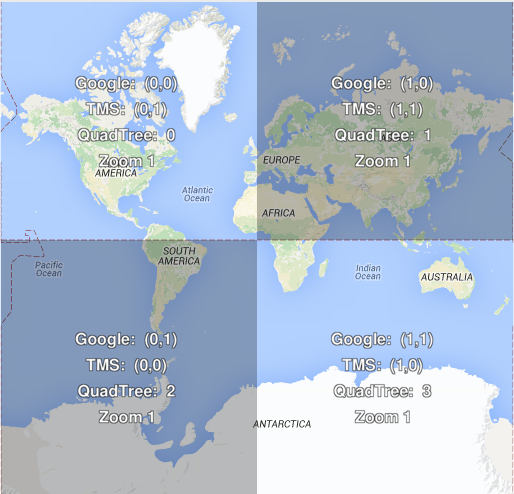
\includegraphics[width=150pt]{images/tiles_a_la_google.png}
	\caption[Tiles à la Google Maps]{Tiles à la Google Maps}
\end{figure}

\subsubsection{QuadKey}
Die \Gls{Quadkeys} von Bing Maps bauen sich wie auf der Abbildung ersichtlich auf. Jedes Zoomlevel führt dazu, dass der QuadKey um eine Stelle zu nimmt. Somit kann die Anzahl der Tiles für das ensprechende Zoomlevel mit dem Zoomlevel als Exponenten zur Basis 4 angegeben werden ($4^{Zoomlevel}$).  \\
\begin{figure}[H]
	\centering
	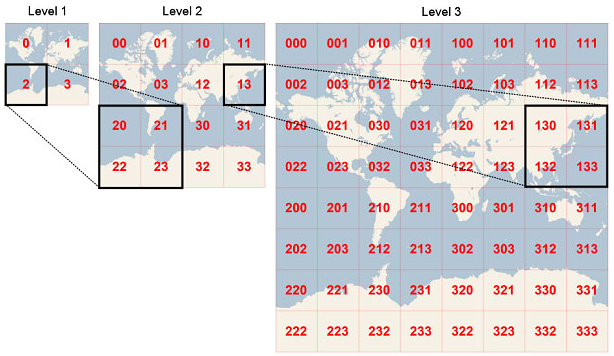
\includegraphics[width=300pt]{images/quadkey.png}
	\caption[QuadTree]{\Gls{QuadTree}}
\end{figure}
\newpage
\subsubsection{Beispiel Code}
Das folgende Beispiel zeigt die Umrechung vom WGS84 Koordinatensystem zu Meter, zu Tiles und schlussendlich zum Quadkey. (Auf dem Zoomlevel 19) \\
\begin{python}
	from src.data.globalmaptiles import GlobalMercator
	
	zoom = 19
	latitude = 47.0
	longitude = 8.0
	mercator = GlobalMercator()
	
	meter_x, meter_y = mercator.LatLonToMeters(latitude, longitude)
	tile_x, tile_y = self._mercator.MetersToTile(meter_x, meter_y, zoom)
	quadkey = mercator.QuadTree(tile_x, tile_y, zoom)
\end{python}




\section{Bilderkennung- detection}

\subsection{Anfertigung der Bilder entlang der Strassen}
Damit das Convnet die Einteilung zwischen Zebrastreifen und Nicht-Zebrastreifen machen kann, braucht es ein RBG Bild mit 50 x 50 Pixeln als Input. Diese Inputbilder werden aus dem gedownloadetem Orthofoto ausgeschnitten. Mithilfe der Strassenkoordinaten muss nicht das ganze Orthofoto in kleine Bilder aufgeteilt, sondern die Inputbilder können nur entlang der Strassen ausgeschnitten werden. Der Abstand zwischen zwei Inputbildern (auch Schrittweite) ist so gewählt, das eine gewisse Überlappung vorliegt.
\\
\decision{Eckdaten Anfertigung Inputbilder} 
Die Inputbilder für das Convnet sind 50 x 50 Pixel gross, da auf Zoomstufe 19 50 Pixel etwa der Breite von zwei Strassen entspricht. Die Schrittweite wurde so angepasst, dass auch Zebrastreifen, die zwischen zwei Inputbildern liegen, erkannt werden.
\\
\begin{figure}[H]
	\centering
	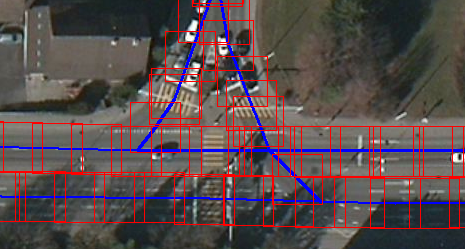
\includegraphics{images/squared_images.png}
	\caption{Blau: Strassenverlauf, Rot: Ausgeschnittene Bilder 50 x 50 Pixel. Diese Visualisierung der Inputbilder kann für jede beliebige BBox selbst durchgeführt werden. Siehe dazu examples/VisualizeSquaredImages.py im Projektordner}
\end{figure}



\subsection{Convnet}
Wir verwenden ein Convolutional Neuronal Network (Convnet) um die automatische Einteilung von Zebrastreifen und Nicht-Zebrastreifen zu machen. Um ein Convnet verwenden zu können, muss man es zuerst mit entsprechendem Bildmaterial trainieren. Wir sprechen hier Inputbilder, welche zum Teil automatisch mithilfe der Open Street Map Datenbank generiert werden konnten, aber meistens von Hand erstellt werden mussten. Wir haben uns während dieses Projektes ein Datenset aus über 4'400 Zebrastreifen- und 32'000 Nicht-Zebrastreifenbilder erarbeitet, um dies zu bewerkstelligen. Diese Arbeit beinhaltete stundelanges Aussortieren von Bildern.
\\

\begin{figure}[H]
	\centering
	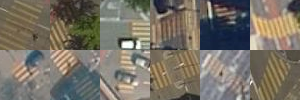
\includegraphics{images/Zebrastreifen_examples.png}
	\caption{6 x 2 Beispiele für Zebrastreifen. Wie auf den Bildern zu sehen ist, verdecken immer wieder Gegenstände das gelbe Muster. Die unterschiedliche Bildqualität der Orthofotos behinderte das Erkennen stark.}
\end{figure}

\begin{figure}[H]
	\centering
	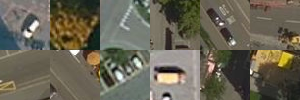
\includegraphics{images/No_Zebrastreifen_examples.png}
	\caption{6 x 2 Beispiele für Nicht-Zebrastreifen. Das Nicht-Zebrastreifen Set beinhaltet alle möglichen Strassensituationen von Stadt bis Land. Besonders bei gelben Autos oder Strassenmarkierungen hat das Convnet mühe.}
\end{figure}

\subsection{Parallelisierung}
\input{chapter/software_dokumentation/api/rq}
\section{Programmierschnittstellen}
\input{chapter/software_dokumentation/api/mapquest}
\input{chapter/software_dokumentation/api/rq}
\input{chapter/software_dokumentation/api/tile_a_la_google}
\section{Test}
\subsection{Unittests}
In der Python Standard Library gibt es das Unit Testing Framework \textbf{unittest}, das es erlaubt Unittests zu implementieren.

\subsubsection{Beispiel Test}
\begin{python}
import unittest
import json, os
from src.role.WorkerFunctions import store, PATH_TO_CROSSWALKS
from src.base.Node import Node

class TestWorkerFunctions(unittest.TestCase):

    def setUp(self):
        self.remove_file()

    def tearDown(self):
        self.remove_file()
        
    def test_store_two_crosswalks(self):
        crosswalks = [Node(47.0, 8.0), Node(47.1, 8.1)]
        store(crosswalks)
        with open(Constants.PATH_TO_CROSSWALKS, 'r') as f:
            data = json.load(f)
        self.assertTrue(len(data['crosswalks']) == 2);
        
    def remove_file(self):
        if os.path.exists(PATH_TO_CROSSWALKS):
            os.remove(PATH_TO_CROSSWALKS) 
\end{python}
\subsection{CircleCI}
\Gls{CircleCI}\cite{circleci} ist ein Tool für Continuous Integration und Deployment, welches wir einsetzten um unsere Tests nach einen Update in unserem Githup Repository automatisch durchzuführen. CircleCI ermöglicht eine Anbindung zu einem Docker Image. Damit konnten wir die vielen Dependencies abdecken, welche unsere Applikation beinhaltet.

\chapter{Projektmanagement}
\section{Entwicklungsumgebung und Infrastruktur}
\subsection{IDE (Integrated Development Environment)}
\decision{PyCharm}	
Beiden Projektmitgliedern ist JetBrains Intellij bekannt und \Gls{PyCharm} ist im Umgang nahe zu identisch.
Für Studenten sind die Entwicklungsumgebungen kostenlos verfügbar.
\subsection{SCM (Source Control Management)}
\decision{GitHub}
Der Umgang mit \Gls{Git} ist beiden Projektmitglieder bestens bekannt.
\Gls{GitHub} ist ohne Unkosten von überall verfügbar
Das Geometalab der HSR publiziert über diesen Weg diverse Projekte

\subsection{CI (Continuous Integration)}
\decision{CircleCI}
Das finden eines passenden Continuous Integration Tools stellte sich schwieriger dar, als zu Beginn des Projektes erwartet. Während dem SE2 Projekt haben wir Bekanntschaft mit Travis CI gemacht, welches die vielen Abhängigkeiten unseres Codes nicht abdecken konnte. Mit CircleCI fanden wir eine Lösung, die auf Docker Hub zugreifen kann, dann den Build des Images durchführt und Schlussendlich die Test durchführt.

\subsection{Projektmanagement Tool}
\decision{Jira}
\Gls{Jira} ist den Projektmitgliedern schon aus dem SE2-Projekt bekannt und hat sich sehr bewährt
Das Dashboard ist übersichtlich gestaltet, es ermöglicht eine Übersicht über die aktuellen Tasks auf einen Blick
Alle Mitglieder haben zu jederzeit Zugriff auf die Plattform, dies erhöht die Transparenz
Weiter bietet Jira diverse Reports um Auswertungen über das Projekt zu fahren.

\section{Planung}
Am Anfang es Projektes haben wir eine grobe Planung zusammengestellt. Dabei haben wir die Phasen und Meilensteine definiert. Während dem Projekt stellten wir immer wieder grössere oder kleinere Abweichungen an der zu Beginn definierten Planung fest. Dieses ist jedoch nicht erstaunlich, da nie absolut korrekt geplant werden kann. Um solche Schwierigkeiten zu handhaben, erstellten wir ein Risikomanagementdokument.

\subsection{Phasen}
\begin{enumerate}
  \item Inception
  \begin{enumerate}
    \item Aufgabenstellung ausarbeiten
  \end{enumerate}
  \item Elaboration1
  \begin{enumerate}
    \item Evaluation der Algorithmen (Bilderkennung)
  \end{enumerate}
  \item Elaboration2
  \begin{enumerate}
    \item Prototyp 1 (in Orthofotos, out Koordinaten)
    \item Prototyp 2 MapRoulett
  \end{enumerate}
  \item Construction1
  \begin{enumerate}
    \item Schnittstelle Satellitenbilder
    \item Optimierungen durch Strassenverlauf und ähnliches
  \end{enumerate}
  \item Construction2
  \begin{enumerate}
    \item Maproulette (Tags und Quiz)
    \item Koordinaten erfassen	
  \end{enumerate}
  \item Transition
  \begin{enumerate}
    \item Dokumentation abschliessen
    \item Challenge auf Maproulette
  \end{enumerate}
\end{enumerate}
\newpage

\subsection{Meilensteine}
\begin{enumerate}
	\item MS1 Algorithmus für Bilderkennung evaluiert
	\item MS2 Prototyp erstellt
	\item MS3 Automatisierte Datenverarbeitung
	\item MS4 Applikation fertiggestellt
	\item MS5 Challenge auf Maproulette
\end{enumerate}

\subsection{Zeitplanung}
Aufwand: 14 Wochen zu 2 * 16 Stunden = \textbf{448 Stunden}
\begin{tabbing}[H]
    \hspace*{6cm}\=\hspace*{6cm}\= \kill
    Inception \>  1 Woche \\
	Elaboration1 \>	3 Wochen \\
	Elaboration2 \>	4 Wochen \\
	Construction1 \> 3 Wochen \\
	Construction2 \> 1 Wochen \\
	Transition \> 2 Wochen \\
\end{tabbing}


\section{Soll-Ist-Zeit-Vergleich}

\subsection{Inception}
\begin{tabbing}[H]
    \hspace*{6cm}\=\hspace*{6cm}\= \kill
    Start: \> 14.09.2015 \\
	Ende: \> 23.09.2015 \\
\end{tabbing}
\begin{figure}[H]
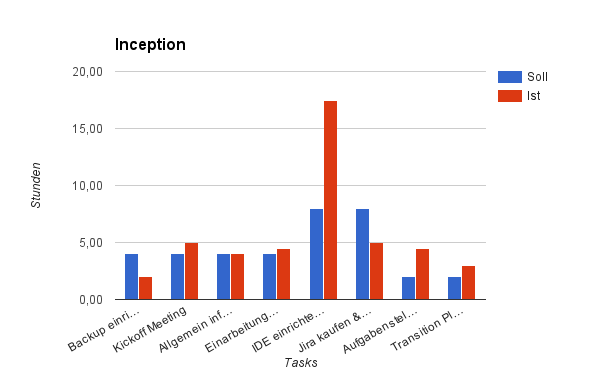
\includegraphics[width=\textwidth]{images/inception.png}
\caption[Inception]{Inception}
\end{figure}

\subsection{Elaboration1}
\begin{tabbing}[H]
    \hspace*{6cm}\=\hspace*{6cm}\= \kill
    Start: \> 23.09.2015 \\
	Ende: \> 19.10.2015 \\
\end{tabbing}
\begin{figure}[H]
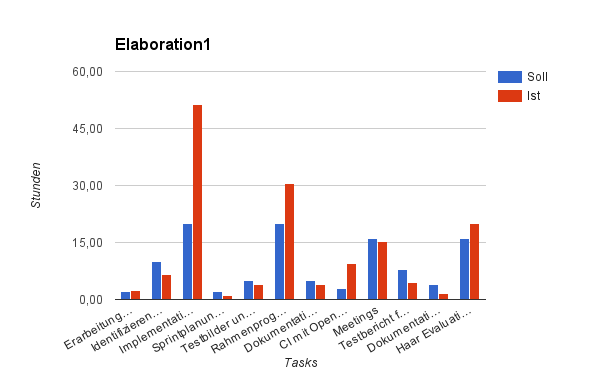
\includegraphics[width=\textwidth]{images/elab1.png}
\caption[Elaboration1]{Elaboration1}
\end{figure}

\subsection{Elaboration2}
\begin{tabbing}[H]
    \hspace*{6cm}\=\hspace*{6cm}\= \kill
    Start: \> 19.10.2015 \\
	Ende: \>  04.11.2015 \\
\end{tabbing}
\begin{figure}[H]
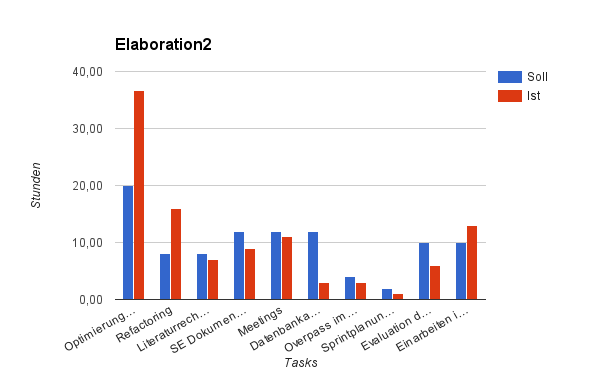
\includegraphics[width=\textwidth]{images/elab2.png}
\caption[Elaboration2]{Elaboration2}
\end{figure}

\subsection{Construction1}
\begin{tabbing}[H]
    \hspace*{6cm}\=\hspace*{6cm}\= \kill
    Start: \> 04.11.2015 \\
	Ende: \>  25.11.2015 \\
\end{tabbing}
\begin{figure}[H]
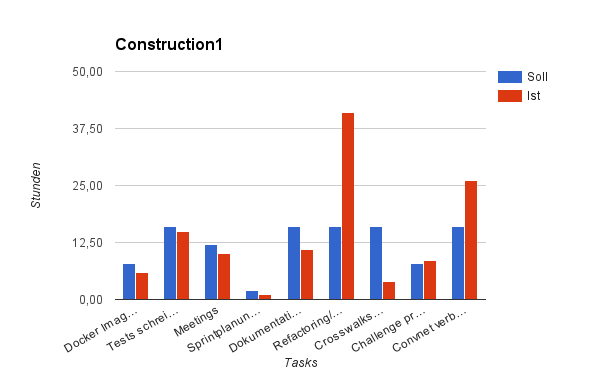
\includegraphics[width=\textwidth]{images/construction1.png}
\caption[Construction1]{Construction1}
\end{figure}

\subsection{Construction2}
\begin{tabbing}[H]
    \hspace*{6cm}\=\hspace*{6cm}\= \kill
    Start: \> 04.11.2015 \\
	Ende: \>  11.11.2015 \\
\end{tabbing}

\subsection{Transition}
\begin{tabbing}[H]
    \hspace*{6cm}\=\hspace*{6cm}\= \kill
    Start: \> 11.12.2015 \\
	Ende: \>  18.12.2015 \\
\end{tabbing}

\subsection{Übersicht}
\begin{table}[H]
    \begin{tabular}{|p{5cm}|p{2cm}|p{2cm}|p{2cm}|}
    \hline    
    \rowcolor{lightblue}
	Phase & Soll & Ist & Differenz \\ \hline
	Inception & 36.00 &	45.50 &	-9.50 \\ \hline
	Elaboration1 & 111.00 & 150.50	& -39.50 \\ \hline
	Elaboration2 & 98.00 & 105.75 & -7.75 \\ \hline
	Construction1 & 110.00 & 122.50 & -12.50 \\ \hline
	\rowcolor{lightblue}
	Total & & & \\ \hline
    \end{tabular}
    \caption[Phasen]{Phasen}
\end{table}

\newpage
\section{Codestatistik}
\subsection{Test Coverage}
Test Coverage wurde mit dem Tool \textbf{nose} durchgeführt. \\

\begin{table}[H]
\centering
    \begin{tabular}{|l|l|}
    \hline    
    \rowcolor{lightblue}
	Datei & Coverage [\%] \\ \hline
	src/base/Bbox.py & 85 \\ \hline    
	src/base/Node.py & 97 \\ \hline   
	src/base/Street.py & 92 \\ \hline  
	src/base/Tile.py & 98 \\ \hline   
	src/base/TileDrawer.py & 24 \\ \hline  
	src/data/MapquestApi.py & 100 \\ \hline   
	src/data/MultiLoader.py & 94 \\ \hline   
	src/data/StreetLoader.py & 100 \\ \hline   
	src/data/TileLoader.py & 100 \\ \hline   
	src/detection/BoxWalker.py & 100 \\ \hline   
	src/detection/NodeMerger.py & 89 \\ \hline  
	src/detection/StreetWalker.py & 100 \\ \hline   
	src/detection/deep/Convnet.py & 97 \\ \hline   
	src/detection/deep/training/Crosswalk\_dataset.py & 100 \\ \hline  
	src/detection/deep/training.py & 100 \\ \hline   
	src/role/Manager.py & 91 \\ \hline  
	src/role/WorkerFunctions.py & 70 \\ \hline
	\rowcolor{lightblue}
	Durchschnitt &   90.5 \\ \hline
    \end{tabular}
    \caption[Test Coverage]{Test Coverage}
\end{table}

\subsection{Codezeilen}
Die Codezeilen wurden mit Hilfe von CLOC \cite{CLOC} ausgezählt. \\

\begin{table}[H]
\centering
    \begin{tabular}{|p{3cm} |p{3cm} |p{3cm} |}
    \hline    
    \rowcolor{lightblue}
	Sprache & Dateien & Zeilen  \\ \hline   
	Python & 43 & 2045 \\ \hline
    \end{tabular}
    \caption[Codezeilen]{Codezeilen}
\end{table}



\chapter{Softwaredokumentation}
\newpage
\section{Installation}
\subsection{Redis}
\label{subsec:redis}
Die Installation wurde auf einem Ubuntu Server durchgeführt, welcher das Paketverwaltungssystem Advanced Packaging Tool (APT) verwendet. Die im Anschluss aufgeführten Befehle werden in einer Shell ausgeführt.
Fals Probleme auftreten bietet Redis ein Quick Start Dokumentation an.

\subsubsection{Installaiton}
\begin{lstlisting}[style=BashInputStyle]
	# sudo apt-get install redis-server
\end{lstlisting}

\subsubsection{Konfiguration}
\begin{lstlisting}[style=BashInputStyle]
	# redis-cli -p 40001
	# CONFIG SET requirepass "crosswalks"
	# redis-cli AUTH crosswalks
\end{lstlisting}

\subsubsection{Starten}
\begin{lstlisting}[style=BashInputStyle]
	# redis-server --port 40001
\end{lstlisting}

\newpage

\subsection{Docker}
\label{subsec:docker}
Die Installaton unserer Applikation beinhaltet diverse Dependencies, welche für die Installation einerseits viel Zeit in Anspruch nehmen und anderseits auch nicht wirklich trivial sind (An dieser Stelle ist Keras zu erwähnen, welches für den Deep Learnig Ansatz verwendet wird). \\
\decision{Docker}
Deshalb haben wir ein Docker Image ersellt, das auf Dockerhub \cite{DokerCrosswalk} frei zur Verfügung gestellt wird und somit den DevOps Prozess massiv vereinfach.\\

\subsubsection{Installaiton}
Bei der Installation von Docker ist zu beachten, dass die Anwendung nur auf 64-Bit Maschinen läuft. Weiter wurden die nachfolgenden Befehle auf Ubuntu durchgeführt und variieren deshalbt zwisch unterschiedlichen Betriebssystemen. 

\paragraph{Vorarbeit}
\begin{lstlisting}[style=BashInputStyle]
	# sudo apt-key adv --keyserver hkp://p80.pool.sks
	-keyservers.net:80 --recv-		
	keys 58118E89F3A912897C070ADBF76221572C52609D
	# echo 'deb https://apt.dockerproject.org/repo ubuntu-precise main' 
	>> /etc/apt/sources.list.d/docker.list
	# apt-get update
	# apt-cache policy docker-engine
	# sudo apt-get install linux-image-extra-$(uname -r)
\end{lstlisting}
\paragraph{Docker installieren}
\begin{lstlisting}[style=BashInputStyle]
	# sudo apt-get install docker-engine
\end{lstlisting}

\subsubsection{Starten}
\begin{lstlisting}[style=BashInputStyle]
	# sudo service docker start
	# sudo docker run hello-world
\end{lstlisting}


\section{Benutzerhandbuch}
\subsection{Suche der Fussgängerstreifen}
Um die Suche der Fussgängerstreifen durchzuführen, muss eine Redis Datenbank zur Verfügung stehen. Weiter muss auf den Rechnern, die als Jobworker tätig sind, Docker installiert sein. \\
Die Installationen sind in folgenden Abschnitten aufgeführt:
\begin{itemize}
	\item Redis:  Abschnitt~\ref{subsec:redis} auf der Seite~\pageref{subsec:redis}
	\item Docker: Abschnitt~\ref{subsec:docker} auf der Seite~\pageref{subsec:docker}
\end{itemize}

\subsubsection{Einführung}
Wir haben unsere Applikation in drei Rollen aufgeteilt:
\begin{itemize}
	\item Manager
	\begin{itemize}
		\item Unterteilt eine grosse Bounding Box in kleinere Boxen mit einer Höhe und Breite von jeweils 2 Kilometern und stellt dies als Jobs in die Queue.
	\end{itemize}
	\item Jobworker
	\begin{itemize}
		\item Arbeite die Jobs der Queue ab.
		\item Gefundene Fussgängerstreifen , welche noch nicht in OpenSteetMap erfasst sind, werden als Job Resultat in die Queue gestellt.
	\end{itemize}
	\item Resultworker
	\begin{itemize}
		\item Schlussendlich werden die Resultate zusammen getragen und in ein JSON File geschrieben.
	\end{itemize}
\end{itemize}

Dieser Ablauf ist genauer beschrieben unter dem Abschnitt~\ref{subsec:ablauf} auf der Seite~\pageref{subsec:ablauf}

\newpage
\subsubsection{Anwendung}
Dank Docker kann unsere Applikation innert Minuten gestartet werden.

\paragraph{Docker Pull}\mbox{}\\
\begin{lstlisting}[style=BashInputStyle]
	# docker pull geometalab/osm-crosswalk-detection
\end{lstlisting}

\paragraph{Manager}\mbox{}\\
\begin{lstlisting}[style=BashInputStyle]
	# docker run geometalab/osm-crosswalk-detection manager
 	  left bottom right top
\end{lstlisting}
Left, Bottom, Right, Top entsprechen den Koordinaten im WGS84 Format. \\
Ostschweiz: left=8.361002, bottom=47.166994, right=8.977610, top=47.706676

\paragraph{Jobworker}\mbox{}\\
\begin{lstlisting}[style=BashInputStyle]
	# docker run geometalab/osm-crosswalk-detection jobworker
\end{lstlisting}
Jobworker können auf beliebig vielen Rechnern gestartet werden.\\

\paragraph{Resultworker}\mbox{}\\
\begin{lstlisting}[style=BashInputStyle]
	# docker run geometalab/osm-crosswalk-detection resultworker
\end{lstlisting}
Die Resultate werden in der Datei crosswalks.json gespeichert. Diese findet man im Verzeichnis in dem der Resultworker gestartet wurde.

\subsubsection{Struktur JSON}
Die Struktur der crosswalks.json Datei ist folgendermassen aufgebaut:
\medskip
\begin{python}
{
	"crosswalks":
	[
		{"latitude": 47.0, "longitude": 8.3},
		{"latitude": 48.0, "longitude": 8.4}
	]
}
\end{python}

\newpage

\subsection{Daten visualisieren}
Um das Resultat des Erkennungsalgorithmus zu visualisieren bot sich das Tool CartoDB \cite{CartoDB} an. Dieses ermöglicht Daten in diversen Formaten hochzuladen und auf einer Karte anzuzeigen.

\subsubsection{Vorgehen}
\begin{enumerate}
	\item Daten (crosswalk.json) mit den Spalten latitude und longitude. in CSV Format umwandeln
	\item CSV Datei in CartoDB als neues Dataset hochladen.
\end{enumerate}

\subsubsection{Struktur CSV}
Die Struktur der CSV Datei gliedert sich wie folgt:
\medskip
\begin{python}
	latitude,	longitude
	47.0,		8.3
	48.0,		8.4
\end{python}


\subsubsection{Daten selektieren}
CartoDB ermöglicht eine Selektion der Daten. So kann zum Beispiel ein Polygon selektiert werden.
\medskip
\begin{python}
SELECT * FROM dataset WHERE ST_WITHIN(
 	ST_Transform(the_geom, 4326), ST_SetSRID(
 	ST_GeomFromGeoJSON('{ "type": "Polygon",
        "coordinates": [
          [ [8.81429672241211,
             47.22971054221563],
            [8.8385009765625,
             47.22877798599878],
            [8.820991516113281,
             47.2185187846731],
            [8.81429672241211,
             47.22971054221563]
          ]
        ] }'),
   4326))
\end{python}
\newpage
\subsection{Challenge erstellen}
Nach dem die Fussgängerstreifen detektiert wurden und die Datei crosswalks.json erstellt wurde, muss dies noch in ein passendes Format für MapRoulette gebracht werden. Dazu haben wir ein Python Skript geschrieben, welches aus jedem gefundenen Fussgängerstreifen einen Task generiert.

\subsubsection{Anwendung}
Für eine Challenge benötigt es die Datei challange.json, welches die Challenge beschreibt und ein zweite Datei tasks.json, in dem sich die Tasks befinden.\\

\paragraph{Tasks generieren}\mbox{}\\
\begin{lstlisting}[style=BashInputStyle]
 # python CrosswalksConverter.py --maproulette crosswalks.json
\end{lstlisting}

\paragraph{Challenge publizieren}\mbox{}\\
\begin{lstlisting}[style=BashInputStyle]
 # curl -u devuser:mylittlesony -vX
   POST http://maproulette.org/api/admin/challenge/
   crosswalk-detection/tasks -d @tasks.json
   --header "Content-Type: application:json"
\end{lstlisting}

\paragraph{Tasks publizieren}\mbox{}\\
\begin{lstlisting}[style=BashInputStyle]
 # curl -u devuser:mylittlesony -vX
   POST http://maproulette.org/api/admin/challenge/
   crosswalk-detection -d @challenge.json
   --header "Content-Type: application:json"
\end{lstlisting}


Als Hilfestellung zum Erstellen von MapRoulette Challanges gibt es ein empfehlenswertes Tutorial \cite{Tutorial}.

\newpage
\subsection{Keras Training}
Für das Training des Neuronalen Netzes steht ein eigenes Docker Image \cite{DokerKeras} auf Docker Hub bereit. Das Image basiert auf einem offiziellen Nvidia Cuda Image und ist fähig mit einer Nvidia Grafikkarte zu arbeiten. Die Grafikkarte wird mit Hilfe des nvidia-docker Projekts geladen. CUDA muss dabei auf dem Host Rechner installiert sein.


\subsubsection{Keras Image}
\paragraph{Download des nvidia-docker Projekts}\mbox{}\\
\begin{lstlisting}[style=BashInputStyle]
	# git clone https://github.com/NVIDIA/nvidia-docker.git
	# cd nvidia-docker
\end{lstlisting}

\paragraph{Herunterladen des Images}\mbox{}\\
\begin{lstlisting}[style=BashInputStyle]
	# docker pull geometalab/keras_cuda
\end{lstlisting}

\paragraph{Start des Containers und mount der Grafikkarte Nummer 0}\mbox{}\\
\begin{lstlisting}[style=BashInputStyle]
	#GPU=0 ./nvidia-docker run -i -t geometalab/keras_cuda /bin/bash
\end{lstlisting}

Achtung: Die Keras Bibliothek entwickelt sich ständig weiter. Auch die Interfaces der populärsten Klassen können sich ändern und haben sich auch schon während diesem Projekt verändert! In diesem Keras Docker Image ist der Stand von Keras installiert, mit dem wir gearbeitet haben. Keras bietet leider keine Versionierung an. Der von uns verwendete Stand ist auch auf der mitglieferten CD erhältlich.

Ein Beispiel für das Training eines Neuronalen Netzes kann in examples/ConvnetTrainer.py und in den Keras eigenen Examples eingesehen werden.

\chapter{Anhang}
\appendix
\newpage
\section{Inhalt der CD}
Der Inhalt der CD glieder sich folgendermassen:
\begin{figure}[H]
\dirtree{%
.1 src/.
.2 detection.
.3 StreetWalker.py.
.3 BoxWalker.py.
.3 NodeMerger.py.
.3 deep.
.4 Convnet.py.
.4 training.
.5 Crosswalk\_dataset.py.
.5 ConvnetTrainer.py.
.2 challenge.
.3 TaskGenerator.py.
.3 run.
.3 tasks.json.
.2 role.
.3 Manager.pyc.
.3 Worker.pyc.
.3 WorkerFunctions.py.
.3 Worker.py.
.3 Manager.py.
.3 main.py.
.2 base.
.3 Tile.pyc.
.3 Tile.py.
.3 Street.py.
.3 Constants.py.
.3 Bbox.py.
.3 Street.pyc.
.3 Bbox.pyc.
.3 Node.py.
.3 TileDrawer.pyc.
.3 TileDrawer.py.
.3 Constants.pyc.
.3 Node.pyc.
.2 data.
.3 StreetLoader.pyc.
.3 TileLoader.py.
.3 MapquestApi.py.
.3 StreetLoader.py.
.3 globalmaptiles.py.
.3 MultiLoader.py.
.3 StreetDrawer.py.
}
\end{figure}


\begingroup     
\let\clearpage\relax        
\printglossary[title=\chapter{Glossar}]
\endgroup
% Bibliography
%%%%%%%%%%%%%%
\bibliographystyle {alpha}
\bibliography{index/bibliography}

\end{document}


\newpage
% List of figures & glossary
%%%%%%%%%%%%%%%%%%%%%%%%%%%%
\listoffigures
\printglossary[style=altlist,title=Glossar]

% Bibliography
%%%%%%%%%%%%%%
\bibliographystyle {alpha}
\bibliography{index/bibliography}


% Attached sources
%%%%%%%%%%%%%%%%%%
 \input{attachments/attachments}


\newpage
\listofdecision

\newpage
\listoftables

\end{document}